\documentclass{standalone}
% font set
\usepackage{ctex}
\usepackage{fontspec}
\usepackage[T1]{fontenc}
\usepackage[sc]{mathpazo}
\usepackage{anyfontsize}
\setmainfont{Source Serif 4}
\setsansfont{Source Sans 3}
\setmonofont{Menlo}
\setCJKmainfont[BoldFont=黑体-简 中等,ItalicFont=楷体-简 常规体]{宋体-简 常规体}

% colors
\usepackage[dvipsnames]{xcolor}
\definecolor{pku-red}{RGB}{139,0,18}
\usepackage{colortbl}
\newcommand{\light}[1]{\textcolor{Orchid}{#1}}
\newcommand{\contrastlight}[1]{\textcolor{TealBlue}{#1}}

% plots
\usepackage{tikz}
\usepackage{tikz-cd}
\usetikzlibrary{arrows}
\usetikzlibrary{arrows.meta,positioning,calc,3d}
\usepackage{pgfplots}
\pgfplotsset{compat=newest}
\tikzset{
    punkt/.style={
        rectangle,
        rounded corners,
        draw=black, very thick,
        minimum height=2em,
        inner sep=6pt,
        text centered,
        fill=gray!30
    }
}

% math package
\let\Bbbk\relax
\usepackage{amsmath}
\usepackage{mathrsfs}
\usepackage{amssymb}
\usepackage{amsfonts}
\usepackage{stmaryrd}
\usepackage{latexsym}
\usepackage{extarrows}
\SetSymbolFont{stmry}{bold}{U}{stmry}{m}{n}
\begin{document}
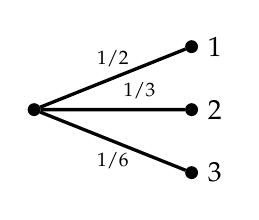
\begin{tikzpicture} [
  level distance=2cm,
  grow'=right,
  level 1/.style= {sibling distance=0.8cm},
  solid node/.style= {circle,draw,inner sep=1.5,fill=black},
  edge from parent/.style={very thick,draw}
]
\node (0) [solid node] {}
  child {node (A1) [solid node,label=right: {$1$}] {} edge from parent node [above] {\scriptsize $1/2$}}
  child {node (A2) [solid node,label=right: {$2$}] {} edge from parent node [above right] {\scriptsize $1/3$}}
  child {node (A3) [solid node,label=right: {$3$}] {} edge from parent node [below] {\scriptsize $1/6$}};
\end{tikzpicture}
\qquad
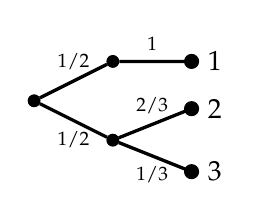
\begin{tikzpicture} [
  level distance=1cm,
  grow'=right,
  level 1/.style= {sibling distance=1cm},
  level 2/.style= {sibling distance=0.8cm},
  solid node/.style= {circle,draw,inner sep=1.5,fill=black},
  edge from parent/.style={very thick,draw}
]
\node (0) [solid node] {}
  child {node (A1) [solid node,label=right: {}] {} 
  child {node (B1) [solid node,label=right: {$1$}] {} edge from parent node [above] {\scriptsize $1$}}
  edge from parent node [above]{\scriptsize $1/2$}
    }
  child {node (A2) [solid node,label=right: {}] {} 
  child {node (B2) [solid node,label=right: {$2$}] {} edge from parent node [above] {\scriptsize $2/3$}}
  child {node (B3) [solid node,label=right: {$3$}] {} edge from parent node [below] {\scriptsize $1/3$}}
  edge from parent node [below] {\scriptsize $1/2$}
  };
  
\end{tikzpicture}
\end{document}